\documentclass[12pt,english,dvipsnames,aspectratio=169,handout]{beamer}\usepackage[]{graphicx}\usepackage[]{xcolor}
% maxwidth is the original width if it is less than linewidth
% otherwise use linewidth (to make sure the graphics do not exceed the margin)
\makeatletter
\def\maxwidth{ %
  \ifdim\Gin@nat@width>\linewidth
    \linewidth
  \else
    \Gin@nat@width
  \fi
}
\makeatother

\definecolor{fgcolor}{rgb}{0.345, 0.345, 0.345}
\newcommand{\hlnum}[1]{\textcolor[rgb]{0.686,0.059,0.569}{#1}}%
\newcommand{\hlstr}[1]{\textcolor[rgb]{0.192,0.494,0.8}{#1}}%
\newcommand{\hlcom}[1]{\textcolor[rgb]{0.678,0.584,0.686}{\textit{#1}}}%
\newcommand{\hlopt}[1]{\textcolor[rgb]{0,0,0}{#1}}%
\newcommand{\hlstd}[1]{\textcolor[rgb]{0.345,0.345,0.345}{#1}}%
\newcommand{\hlkwa}[1]{\textcolor[rgb]{0.161,0.373,0.58}{\textbf{#1}}}%
\newcommand{\hlkwb}[1]{\textcolor[rgb]{0.69,0.353,0.396}{#1}}%
\newcommand{\hlkwc}[1]{\textcolor[rgb]{0.333,0.667,0.333}{#1}}%
\newcommand{\hlkwd}[1]{\textcolor[rgb]{0.737,0.353,0.396}{\textbf{#1}}}%
\let\hlipl\hlkwb

\usepackage{framed}
\makeatletter
\newenvironment{kframe}{%
 \def\at@end@of@kframe{}%
 \ifinner\ifhmode%
  \def\at@end@of@kframe{\end{minipage}}%
  \begin{minipage}{\columnwidth}%
 \fi\fi%
 \def\FrameCommand##1{\hskip\@totalleftmargin \hskip-\fboxsep
 \colorbox{shadecolor}{##1}\hskip-\fboxsep
     % There is no \\@totalrightmargin, so:
     \hskip-\linewidth \hskip-\@totalleftmargin \hskip\columnwidth}%
 \MakeFramed {\advance\hsize-\width
   \@totalleftmargin\z@ \linewidth\hsize
   \@setminipage}}%
 {\par\unskip\endMakeFramed%
 \at@end@of@kframe}
\makeatother

\definecolor{shadecolor}{rgb}{.97, .97, .97}
\definecolor{messagecolor}{rgb}{0, 0, 0}
\definecolor{warningcolor}{rgb}{1, 0, 1}
\definecolor{errorcolor}{rgb}{1, 0, 0}
\newenvironment{knitrout}{}{} % an empty environment to be redefined in TeX

\usepackage{alltt}
\usepackage{fontspec}
\setsansfont[Mapping=tex-text]{Fira Sans}
\setcounter{secnumdepth}{4}
\setcounter{tocdepth}{4}
\usepackage[normalem]{ulem}
\usepackage[T1]{fontenc}
\usepackage{dcolumn}
\usepackage{booktabs}
\usepackage{bm}
\usepackage{setspace}
\makeatletter
\usetheme{metropolis}
\setbeamertemplate{frame footer}{Bosancianu | Schaub | Hertie School}
\setbeamerfont{page number in head/foot}{size=\tiny}
\setbeamercolor{footline}{fg=gray}
\usepackage{xcolor}
\setbeamercovered{transparent}
\usepackage{tikz}
\usetikzlibrary{arrows, positioning}
\usepackage[labelformat=empty]{caption}
% For table captions in Beamer
\usepackage[sectionbib]{apacite}
\renewcommand{\bibliographytypesize}{\footnotesize}
\makeatletter
\let\st@rtbibsection\@bibnewpage
\let\st@rtbibchapter\@bibnewpage
\makeatother
\usepackage{amsmath, mathtools}
\usepackage{xunicode}
\usepackage{hyperref}
\graphicspath{{./figures/}} 
% Defines a checkmark
\def\checkmark{\tikz\fill[scale=0.4,color=orange](0,.35) -- (.25,0) -- (1,.7) -- (.25,.15) -- cycle;}
% wide itemize and enumerate
\newenvironment{wideitemize}{\itemize\addtolength{\itemsep}{.3em}}{\enditemize}
\newenvironment{wideenumerate}{\enumerate\addtolength{\itemsep}{.3em}}{\endenumerate}
% boxes
\def\boxitorange#1{%
  \smash{\color{orange}\fboxrule=1pt\relax\fboxsep=2pt\relax%
  \llap{\rlap{\fbox{\vphantom{0}\makebox[#1]{}}}~}}\ignorespaces
}
\def\boxitblue#1{%
  \smash{\color{blue}\fboxrule=1pt\relax\fboxsep=2pt\relax%
  \llap{\rlap{\fbox{\vphantom{0}\makebox[#1]{}}}~}}\ignorespaces
}
\newcommand{\indep}{\perp \!\!\!\! \perp}
\setbeamertemplate{itemize items}{\checkmark}
\usepackage{multirow}
\hypersetup{pdfauthor={Bosancianu and Schaub},
	pdftitle={Statistical Modeling and Causal Inference with R},
	pdfsubject={Week 5: Instrumental variable estimation},
	pdfkeywords={Berlin, Hertie, 2020, week 5}}
\title{\textsc{Statistical Modeling and Causal Inference with R}}
\subtitle{Week 5: Instrumental variable estimation}
\date{October 5, 2020}
\author{Manuel Bosancianu \hfill Max Schaub}
\institute{Hertie School of Governance}
\IfFileExists{upquote.sty}{\usepackage{upquote}}{}
\begin{document}
\maketitle


\begin{frame}
	\frametitle{Lecture Q\&A}
	\begin{itemize} \large
		\item Open Q\&A 
		\item Acemoglu, Johnson, and Robinson \citeyear{acemoglu_colonial_2001}
	\end{itemize}
\end{frame}


\begin{frame}
	\frametitle{Acemoglu, Johnson, and Robinson \citeyear{acemoglu_colonial_2001}: Impact}
	 \begin{figure} 
    
\includegraphics[height=.4\textheight]{../04-figures/05/08-ajr_cites}
    \vfill
    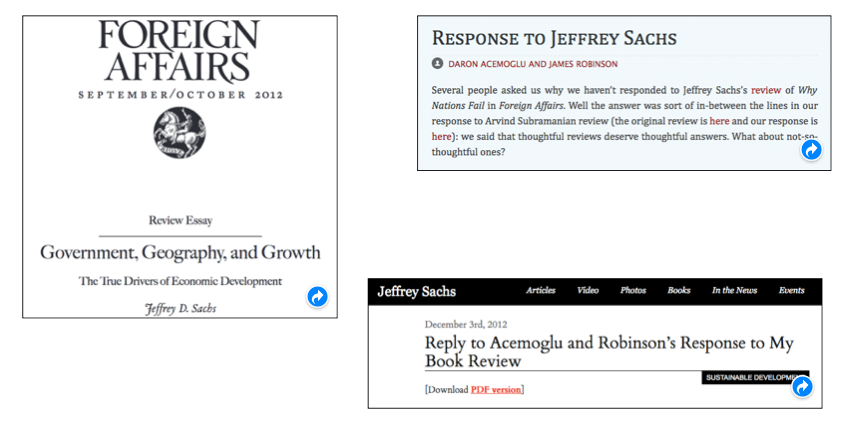
\includegraphics[height=.4\textheight]{../04-figures/05/09-ajr_debate}
    \end{figure}
\end{frame}


\begin{frame}
	\frametitle{Acemoglu, Johnson, and Robinson \citeyear{acemoglu_colonial_2001}: Discussion topics}
	\begin{itemize}
		\item Hypothesis? 
		\item DAG?
		\item Exclusion restriction?
		\item Confounders vs.\ violations of exclusion restriction?
		\item Who are the compliers? 
		\item Possible falsification tests?
	\end{itemize}
\end{frame}


\begin{frame}
	\frametitle{Acemoglu, Johnson, and Robinson \citeyear{acemoglu_colonial_2001}: DAG}
	 \begin{figure} 
    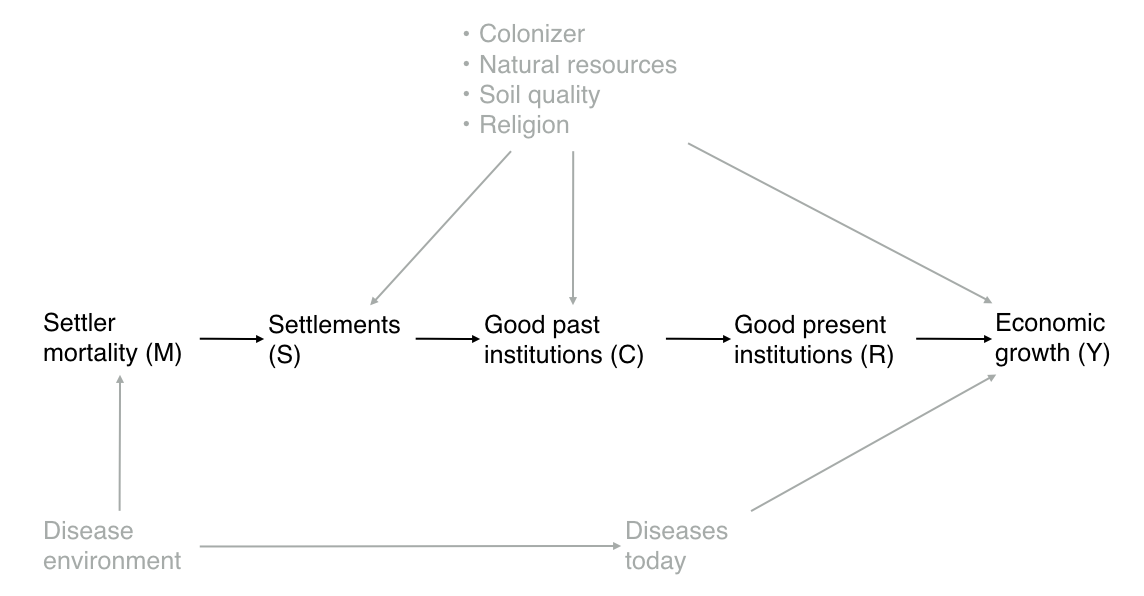
\includegraphics[height=.8\textheight,keepaspectratio=true]{../04-figures/05/10-ajr_dag}
    \end{figure}
\end{frame}


\begin{frame}
	\frametitle{Acemoglu, Johnson, and Robinson \citeyear{acemoglu_colonial_2001}: Exclusion restriction}
	 \begin{figure} 
    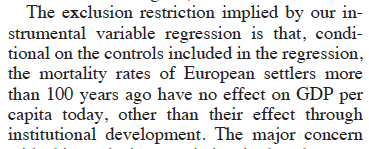
\includegraphics[height=.5\textheight,keepaspectratio=true]{../04-figures/05/11-ajr_er}
    \end{figure}
\end{frame}


\begin{frame}
	\frametitle{Acemoglu, Johnson, and Robinson \citeyear{acemoglu_colonial_2001}: Exclusion restriction?}
	 \begin{figure} 
    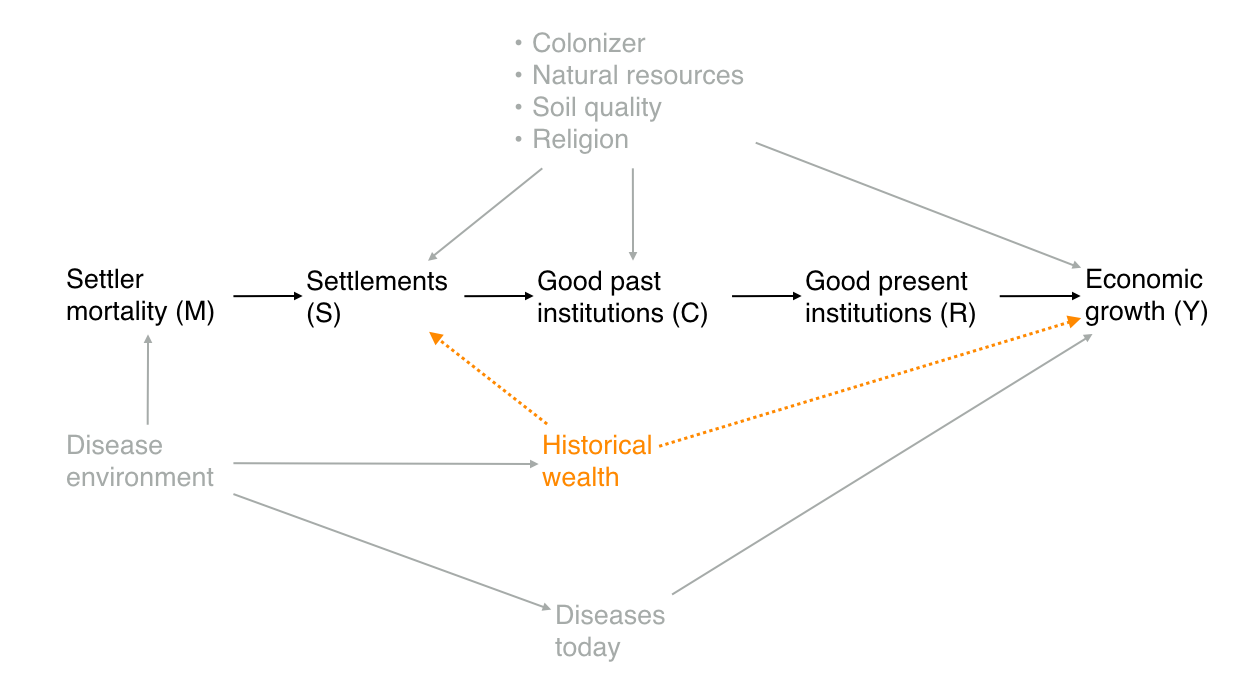
\includegraphics[height=.9\textheight,keepaspectratio=true]{../04-figures/05/12-ajr_dag_crit}
    \end{figure}
\end{frame}


\begin{frame}
	\frametitle{Acemoglu, Johnson, and Robinson \citeyear{acemoglu_colonial_2001}: IV estimates}
	 \begin{figure} 
    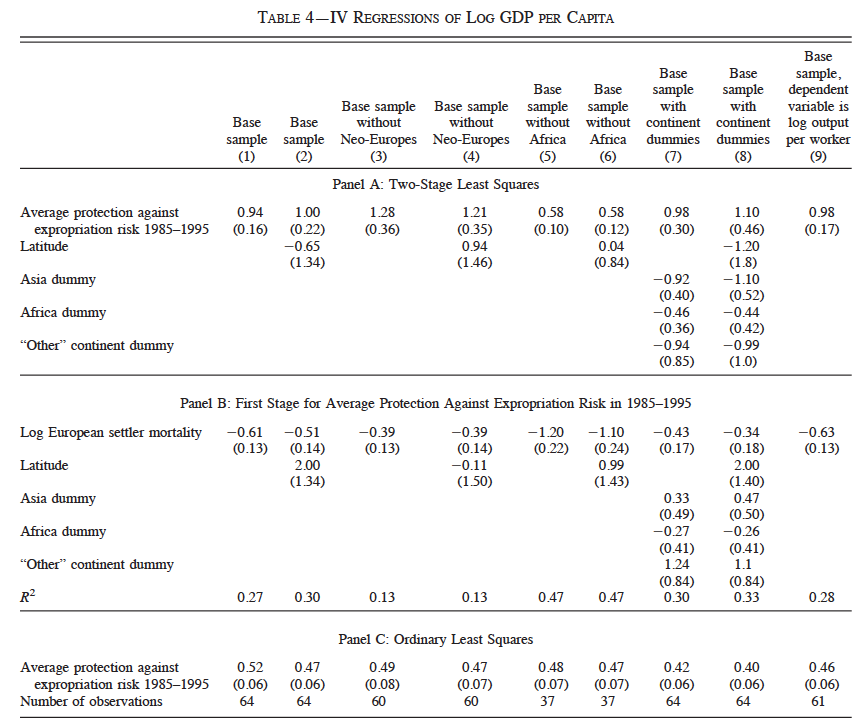
\includegraphics[height=.8\textheight,keepaspectratio=true]{../04-figures/05/13-ajr_table4}
    \end{figure}
\end{frame}


\begin{frame}
	\frametitle{Acemoglu, Johnson, and Robinson \citeyear{acemoglu_colonial_2001}: Latitude comment}
	 \begin{figure} 
    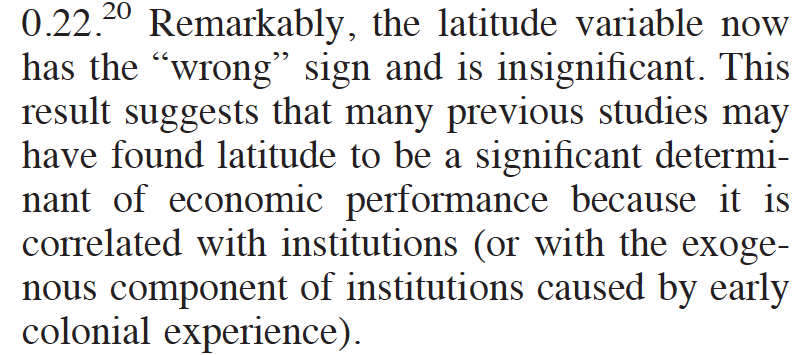
\includegraphics[height=.5\textheight,keepaspectratio=true]{../04-figures/05/14-ajr_latitude}
    \end{figure}
\end{frame}


% END
\begin{frame}
\begin{center}
    \LARGE Thank you for watching, and see you next Monday!
\end{center}
\end{frame}

% REFERENCES %

\begin{frame}[allowframebreaks]
\frametitle{References}
\bibliographystyle{apacite}
\scriptsize\bibliography{../Bibliography}
\end{frame}

\end{document}
